\documentclass[spanish]{beamer}
\usepackage[spanish]{babel} %esto es para que las ondas estn en espaol

% Vary the color applet  (try out your own if you like)
%\colorlet{structure}{red!65!black}

%\beamertemplateshadingbackground{yellow!100}{white}

\usepackage[utf8x]{inputenc}
\usetheme{Madrid} 

\usepackage{beamerthemesplit}
\usepackage{graphics}
\usepackage{graphicx}
\usepackage{hyperref}

\title[El sistema operativo Linux ]{El sistema operativo Linux}
\author[Hector Hurtarte,Carlos L\'{o}pez Camey]{%
  Hector Hurtarte \and
  Carlos L\'{o}pez Camey}
\institute[Florida State University]{
  CC3008 - Sistemas Operativos Avanzados \\
  Departamento de Ciencias de la Computaci\'{o}n \\
  Universidad del Valle de Guatemala}
\date[Investigaci\'{o}n 1]{Investigaci\'{o}n 1}
\subject{Computational Sciences}

%\pgfdeclaremask{fsu}{fsu_logo_ybkgrd}
%\pgfdeclareimage[mask=fsu,width=1cm]{fsu-logo}{fsu_logo_ybkgrd}

%\logo{\vbox{\vskip0.1cm\hbox{\pgfuseimage{fsu-logo}}}}

\begin{document}

  \frame
  {
    %\tableofcontents
    \titlepage
  }

  	\section{Generalidades del dise\~{n}o}
	\subsection{Generalidades del diseño}
  \frame
  {
    \frametitle{Generalidades del diseño}
	Linux es:	
	\begin{itemize}
		\item Multiusuario
		\item Multitarea
		\item Compatible con UNIX (herramientas)
		\item Filesystem Hierarchy Standard 
	\end{itemize}
  }
	\subsection{Estandarización}
	\frame
	{
		\frametitle{Estandarización}	
		\begin{itemize}
		\item Objetivo de importancia para un S.O.: implementación de estándares
		\item Linux busca: velocidad, eficiencia y \textbf{Estandarización}
		\begin{itemize}
			\item POSIX: define comportamientos (Linux-FT sobre POSIX.1)
			\item Linux Standard Base (LSB)
			\begin{itemize}
				\item Jerarquía del sistema de archivos
				\item Bibliotecas estándar
				\item \textit{X Window System}
				\item Críticas: Debian, RPM, pruebas de conformidad
			\end{itemize}
		\end{itemize}
		\item Linux soporta: 
			\begin{itemize}
				\item POSIX: Threads
				\item POSIX: control de procesamiento en tiempo real (subconjunto)
			\end{itemize}
		\end{itemize}
	}
	
	\subsection{Componentes de un sistema Linux}
	\frame
	{
		\frametitle{Componentes de un sistema Linux}	
		Linux está compuesto por:
		\begin{itemize}
			\item Kernel: abstracción para memoria virtual y procesos. 
				\begin{itemize}
					\item Provee funcionalidad para \textbf{ejecución de procesos}
					\item Provee servicios para acceso seguro y arbitrario a recursos hardware
				\end{itemize}
			\item Bibliotecas del sistema
				\begin{itemize}
					\item Proveen interacción aplicación \textit{kernel}
					\item Funcionalidad del S.O. que \textbf{no} necesita privilegios del modo kernel
					\item \textit{System calls} involucran transferencia de control y argumentos
					\item Versiones más complejas (archivos con \textit{buffer} en C) o no correspondidas con llamadas (ordenación, funciones mat.)
				\end{itemize}
			\item Utilidades del sistema
				\begin{itemize}
					\item Tareas individuales y especializadas
					\item Aspectos de configuraci\'{o}n y demonios
				\end{itemize}
		\end{itemize}
	}	
	
	\subsection{Modo kernel}
	\frame
	{
		\frametitle{Modo kernel}
		Lo más importante es notar diferencia entre \textit{kernel} y demás. El \textbf{modo kernel}:
		\begin{itemize}
			\item Modo privilegiado del procesador
			\item Acceso a todos los recursos físicos
			\item Diseño monolítico: S.O. trabaja en espacio de memoria del \textit{kernel}. Mejora \textit{performance}:
			\begin{itemize}
				\item Código y estructuras en mismo espacio de memoria
				\item No se necesitan \textit{context switches} en proceso-S.O. o interrupciones.
			\end{itemize}
		\end{itemize}
	}
	
  	\section{Caracter\'{i}sticas}
	\subsection{Perspectiva del usuario}
  \frame
  {
    \frametitle{Desde la perspectiva usuario}

    \begin{itemize}
      \item Multi-tarea: varios programas pueden correr al \textit{mismo tiempo}
      \item Multi-usuario: varios usuarios pueden tener la sesión iniciada al mismo tiempo.
      \item Multi-plataforma: corre en diferentes procesadores, no sólo Intel.
      \item Multi-procesador: soporte de multi-procesamiento simétrico en las plataformas Intel y SPARC (dos diferentes procesadores compartiendo la misma memoria)
      \item Multi-hilo: soporte para múltiples hilos de control en un cada uno de los espacios de memoria de un proceso.
    \end{itemize}
  }

    \subsection{Perspectiva del desarrollador}
  \frame
  {
    \frametitle{Desde la perspectiva desarrollador}    
    \begin{itemize}
    \item Protección de memoria entre procesos
    \item Memoria virtual usando pagineo a disco: pagineo a una partición u otro sistema de archivos, con la posibilidad de añadir más espacio de $swapping$ en tiempo de corrida.
    \item Piscina de memoria unificada: para programas de usuario y cache de disco (para poder aprovechar la memoria libre para cache o reducir el cache cuando se están corriendo programas $grandes$.
    \end{itemize}
  }

  \frame{
    \frametitle{Desde la perspectiva desarrollador}
    \begin{itemize}
    \item Librer\'{i}as ligadas dinámicamente compartidas (DLL's) y librerías estáticas, generalmente de GNU.
       \item Compatible con POSIX a nivel de código fuente.
       \item Soporte para diferentes sistemas de archivos.
       \item Manejador de LAN (con SMB)
       \item Diferentes protocolos de red
    \end{itemize}
  }

  \section{Historia}
	\subsection{Historia}
  \frame
  {
    \frametitle{Historia}
    \begin{itemize}
    	\item Linus Torvalds, Finlandia, 1991: \textit{kernel} para 80386
    	\item Puesto a disposición en internet
    	\item Distinción \textit{kernel} de Linux vs. Sistema Linux
    \end{itemize}
  }

\subsection{Versi\'{o}n 0.01}
  \frame
  {
    \frametitle{Versi\'{o}n 0.01}
    \begin{itemize}
    	\item 14 de Mayo de 1991
    	\item Procesadores Intel compatibles con 80386 y hardware PC. Limitado soporte para controladores
    	\item Subsistema de memoria virtual básico. Soporte para utilización de páginas compartidas, copia durante escritura*
    	\item \'{U}nico sistema de archivos: Minix (Tanembaum, curso de desarrollo de S.O. Vrije Universiteit, Ámsterdam)
    	\item Implementación de procesos UNIX con espacios de direcciones protegidos
    \end{itemize}
  }
  
\subsection{Versi\'{o}n 1.0}
  \frame
  {
    \frametitle{Versi\'{o}n 1.0}
    \begin{itemize}
    	\item Lanzada en 1994
    	\item Conexiones por red: soporte para TCP/IP de UNIX e interfaz \textit{socket} compatible con BSD. Soporte para dispositivos IP sobre Ethernet
    	\item Permitía paginación sobre archivos de intercambio (swap) y mapeo a memoria de archivos arbitrarios (solo lectura)
    	\item Emulación de coma flotante para procesadores sin coprocesador matem\'{a}tico (intel 80387).
    \end{itemize}
    Luego de esto, desarrollo de 1.1:
    \begin{itemize}
    	\item Est\'{a}ndar de numeraci\'{o}n
    \end{itemize}
  }  
  
  \subsection{Versi\'{o}n 1.2}
  \frame
  {
    \frametitle{Versi\'{o}n 1.2}
    \begin{itemize}
    	\item Soporte a mayor variedad de dispositivos (incluyendo PCI).
    	\item Modo virtual 8086 de CPU 80386 para emular DOS
    	\item Soporte parcial para SPARC, Alpha y MIPS.
    \end{itemize}
  } 

\subsection{Versi\'{o}n 2.0}
  \frame
  {
    \frametitle{Versi\'{o}n 2.0}
    \begin{itemize}
    	\item Lanzada en Junio de 1996
    	\item Dos características principales:
    		\begin{itemize}
    			\item Soporte para múltiples arquitecturas, incluyendo alpha para 64 bits.
    			\item Soporte para arquitecturas multiprocesador
    		\end{itemize}
    	\item Además:
    		\begin{itemize}
				\item Mejoró gestión de memoria (\textit{caché} para datos de \textit{filesystem} indep. de dispositivos de bloque)
				\item Este mecanismo \textit{caché} a archivos de red y mapeados en memoria (modo escritura)
				\item \textit{Performance} de comunicaciones TCP/IP (AppleTalk, AX.25, entre otros)
				\item Capacidad de montar software de red remoto y vol\'{u}menes SMB
				\item \textit{Threads} internas del \textit{kernel} para gestionar dependencias entre m\'{o}dulos
    		\end{itemize}
    \end{itemize}
  } 
  
  \subsection{Versi\'{o}n 2.2}
  \frame
  {
    \frametitle{Versi\'{o}n 2.2}
    \begin{itemize}
    	\item Lanzada en Enero de 1999
    	\item Se añade versión para UltraSPARC
		\item Características de red: \textit{firewall} más flexible, mejores mecanismos de gestión de tráfico
		\item Soporte para ventanas de transmisión TCP
		\item Se mejoro el NFS (nivel de aplicación OSI para sistemas distribuídos) añadiendo demonio en modo \textit{kernel}
		\item Se rediseñaron mecanismos de bloqueo para señales, interrupciones y algunas I/O utilizando granularidad más fina
		\item Mejorar velocidad de SMP
    \end{itemize}
  }  

  \subsection{Versiones 2.4 y 2.6}
  \frame
  {
    \frametitle{Versiones 2.4 y 2.6}
    \begin{itemize}
    	\item Incluyen mayor soporte para SMP, mejoras en gestión de memoria y planificador de procesos con algoritmo \textit{O}(1).
    	\item Permite desalojar proceso mientras modo \textit{kernel}
		\item En concreto \textbf{vesión 2.6}:
		\begin{itemize}
			\item Inició soporte para dispositivos incrustados. $\mu$CLinux (iPodLinux).
			\item \textit{Non-uniform memory access}, la memoria se accede en posiciones relativas a otro procesador o compartida. Adelanto a SMP.
			\item Soporte para \textit{hiperthreading}: un solo procesador enmascara otros a nivel de hardware. \textit{Performance} vs. Complejidad en calendarizaci\'{o}n
		\end{itemize}
    \end{itemize}
  }  
  
 \section{Manejo de procesos}
 
 \subsection{Estándar de POSIX}
 
  \frame
  {
    \frametitle{Modelo \textit{fork()} y \textit{exec()}}

    El estándar de POSIX define dos operaciones sobre procesos
    \begin{itemize}
      \item Creación de procesos con $fork()$
      \item Ejecución de procesos con $exec()$
    \end{itemize}

    Son independientes una de otra:
    \begin{itemize}
      \item Un proceso puede ser creado sin ser ejecutado
      \item Un proceso puede ser ejecutado sin crear uno nuevo
        \begin{itemize}
          \item \textit{proceso.exec()} deja de ejecutar al proceso actual y ejecuta \textit{proceso} en el mismo contexto.
        \end{itemize}
    \end{itemize}
  }

  \frame{
    \frametitle{Abstracción de la información sobre un proceso}
    Un proceso abarca toda la información que el S.O necesita para manejar su contexto con:
    \begin{itemize}
      \item Identidad 
      \item Ambiente
      \item Personalidad
    \end{itemize}
  }

  \subsection{Identidad de un proceso}
  \frame{
    \frametitle{Identidad de un proceso}

    \begin{itemize}
    \item \textbf{PID:} Identificador único, usado para especificar procesos cuando una aplicaci\'{o}n hace una llamada al sistema operativo para efectuar una operaci\'{o}n sobre alg\'{u}n proceso.

    \item \textbf{Credenciales: } Uno o varios identificadores que correspoden al usuario o al grupo que determinan los derechos/permisos de un proceso.  
    \item \textbf{Personalidad: } Identificador que permite modificar la sem\'{a}ntica de ciertas llamadas al S.O. No com\'{u}n en UNIX pero si en Linux.
    \end{itemize}
  }
  
  \subsection{Ambiente de un proceso}
  \frame{
    \frametitle{Ambiente de un proceso}
    Es heredado del padre y está compuesto por dos vectores/listas
    \begin{itemize}
     \item \textbf{Vector de argumentos: } contiene los argumentos de la linea de comando que fueron usados para invocar al programa 
       \begin{itemize}
         \item \textit{cp -R /path/arg1 /path/arg2}
       \end{itemize}

     \item \textbf{Vector de ambiente: } contiene pares de la forma NOMBRE=VALOR, que asocian variables de ambiente con cadenas arbitrarias de texto
       \begin{itemize}
         \item CLASSPATH=/home/user/lib/*.jar
       \end{itemize}
    \end{itemize}
  }

  \subsection{Contexto de un proceso}
  \frame{
    \frametitle{Contexto de un proceso}
    La identidad y ambiente de un proceso son típicamente establecidos cuando un proceso es craedo. El contexto de un proceso es el el $estado$ del mismo en un momento dado:
    \begin{itemize}
    \item \textbf{Contexto de calendarizaci\'{o}n: }
      \begin{enumerate}
      \item Copias de los registros de un proceso. 
      \item Prioridad.
      \item Se\~{n}ales que est\'{a}n esperando ser entregadas al proceso.
      \item Pila del kernel:  área separada de memoria reservada usada exclusivamente en modo kernel. 
        \begin{itemize}
          \item Útil para llamadas al sistema operativo e interrupciones que ocurren cuando el proceso se est\'{a} ejecutando.
        \end{itemize}
  \end{enumerate}
\end{itemize}
  }

  \frame{
    \frametitle{Contexto de un proceso}
    \begin{itemize}
    \item \textbf{Contabilidad: } Informaci\'{o}n sobre los recursos que están siendo consumidos por el proceso y el total de recursos que el proceso ha utilizado.
    \item \textbf{Tabla de archivos: } Arreglo de punteros a estructuras de archivo del kernel, 
      \begin{itemize}
      \item En una operación de I/O, el proceso se refiere a los archivos usando el \'{i}ndice correspondiente en este arreglo.
      \end{itemize}
    \item \textbf{Contexto en el sistema de archivos: } Archivos que están siendo usados por el proceso: 
      \begin{itemize}
        \item Archivos abiertos
        \item Archivos que puede utilizar en un futuro.
        \end{itemize}   
    \end{itemize}
  }

  \frame{
    \frametitle{Contexto de un proceso}

    \begin{itemize}
    \item \textbf{Tabla de manejador de se\~{n}ales}: Define que rutina del proceso llamar cuando una se\~{n}al le sea entregada.
      \begin{itemize}
        \item Puntero a la rutina
      \end{itemize}
    \item \textbf{Contexto en memoria virtual: } Informaci\'{o}n sobre el contenido del espacio de direcciones privado de un proceso.
    \end{itemize}
  }

  \subsection{Procesos y threads}
  \frame{
    \frametitle{Procesos y \textit{threads}}

    Creación de $threads$ con $flags$ específicas con $clone()$:
    \begin{center}
      \begin{tabular}{|c |c |}
        \hline
        Bandera & Significado\\
        \hline
        CLONE\_FS & Se comparte la informaci\'{o}n del sistema de archivos.\\
        CLONE\_VM & Se comparte el espacio de memoria. \\
        CLONE\_SIGHAND & Se comparten los manejadores de se\~{n}ales. \\
        CLONE\_FILES & Se comparte el conjunto de archivos abiertos. \\
        \hline
      \end{tabular}
    \end{center}

    Una llamada a $clone()$ sin ninguna bandera establecida, simularía la funcionalidad de un $fork()$.
  }

  \section{Manejo de memoria}
	\subsection{Manejo de memoria}
  \frame
  {
    \frametitle{Manejo de memoria}
    Linux es sistema de memoria virtual: las direcciones vistas por los programas no deben corresponder a direcciones fijas.
    \begin{itemize}
    	\item Memoria física
    	\item Memoria virtual
    \end{itemize}
  }
  
  \subsection{Memoria física}
  \frame{
	\frametitle{Memoria física}
	Encargado de asignación/liberación: páginas, grupos de páginas y pequeños bloques de memoria.
	Memoria separada en 3 \textbf{zonas}:
	\begin{itemize}
	\item \url{ZONE_DMA}: Utilizada por dispositivos ISA que solo pueden acceder a cantidades limitadas usando DMA.
	\item \url{ZONE_NORMAL}: Mapeada sobre espacio de direcciones de CPU.
	\item \url{ZONE_HIGHMEM}: No mapeada sobre espacio de direcciones del \textit{kernel}. Se reserva para páginas de procesos de usuario.
	\end{itemize}
  }
  
  \frame{
  	\frametitle{Memoria física}
  	\begin{itemize}
  		\item Cada zona tiene \textbf{asignador de páginas}. 
  		\item Utiliza \textit{buddy system} (descomposición binaria)
  		\item Listas encadenadas para control de regiones libres de cada tamaño (min. una página).
  		\item Existen mecanismos que no usan este asignador:
  		\begin{itemize}
  			\item \textbf{kmalloc()}: Asigna páginas pero las descompone en fragmentos.
  			\item \textbf{Slab allocator}: estructuras las del \textit{kernel} y p\'{a}ginas contiguas. \textit{Cach\'{e}s} compuestas de \textit{slabs} para cada estructura (semaforos, descr. de procesos \url{struct} \url{task_struct},etc).
  			\item \textbf{Caché para páginas pertenecientes a archivos}: dispositivos de bloque y archivos mapeados a memoria. I/O. Páginas completas y datos relacionados con la comunicación de red.
  		\end{itemize}
  	\end{itemize}
  }

	\subsection{Memoria virtual}
	\frame{
		\frametitle{Memoria virtual}
		\begin{itemize}
			\item Gestiona memoria mapeada
			\item Crea páginas de memoria virtual
			\item Maneja carga desde memoria o \textit{swap}. 
		\end{itemize}
	}  
  
	\frame{
		\frametitle{Memoria virtual}
		Mantiene dos \textbf{vistas del espacio de direcciones} de un proceso:
		\begin{itemize}
			\item \textbf{Conjunto de regiones separadas}: Espacio de direcciones consiste en un conjunto de regiones modelada por un \url{vm_area_struct} que describe permisos en la regi\'{o}n. \begin{itemize}\item Arbol binario balanceado (búsqueda de dirección virtual)\end{itemize}
			\item \textbf{Conjunto de páginas}: tablas de p\'{a}ginas hardware del proceso que determinan la direcci\'{o}n f\'{i}sicas exacta. Se gestiona por un conjunto de rutinas invocadas desde las interrupciones software del \textit{kernel} (\textit{page faults}). 
		\end{itemize}
	} 
	
	\frame{
		\frametitle{Regiones de memoria virtual}
		Criterios:
		\begin{itemize}
			\item Almacenamiento de respaldo:
				\begin{itemize}
					\item Archivo: visor de secci\'{o}n de archivo (compartir p\'{a}ginas de memoria f\'{i}sica)
					\item Nada: memoria demandada con ceros
				\end{itemize}
			\item Reacci\'{o}n frente a escrituras: el mapeado de una regi\'{o}n sobre espacio de dir. de proc. puede ser:
				\begin{itemize}
					\item Privado: la escritura genera copias para que cambios sigan siendo locales
					\item Nada: provocan que se actualice el objeto mapeado
				\end{itemize}
		\end{itemize}
	} 
	
	\frame{
		\frametitle{Duraci\'{o}n de un espacio de direcciones}
		El \textit{kernel} crea nuevos espacios de direcciones en:
		\begin{itemize}
			\item \url{exec()}: al proceso se asigna nuevo espacio de direcciones vac\'{i}o
			\item \url{fork()}: crea copia de espacio de direcciones virtual del padre.
				\begin{itemize}
					\item \textit{Kernel} copia descriptores \url{vm_area_struct} 
					\item Nada: Crea conjunto de tablas de p\'{a}ginas del hijo y se incrementa
					\item El padre y el hijo comparten p\'{a}ginas fisicas
					\item Caso especial: p\'{a}ginas privadas
					\begin{itemize}
						\item \textit{read-only}: cambios locales. Modificaciones crean copias.
						\item P\'{a}ginas privadas compartidas siempre que sea posible
					\end{itemize}
				\end{itemize}
		\end{itemize}
	}
	
	\frame{
		\frametitle{Paginación y \textit{swapping}}
		\begin{itemize}
			\item Linux utiliza mecanismo de paginación. 
			\item ¿Qué páginas escribir en disco? Algoritmo \textit{second chance} (FIFO, bit de referencia).
			\item Cada p\'{a}gina tiene \textit{edad} ajustada en cada revisi\'{o}n (juventud y actividad)
			\item \textit{Edad} permite seleccionar p\'{a}ginas para sacar seg\'{u}n \textit{last frequently used}
		\end{itemize}
	}
	
  
  \section{Sistema de archivos}
    
  \frame
  {
    \frametitle{Estándar de UNIX}

    Un archivo no es necesariamente un objeto almacenado en disco
    \begin{itemize}
      \item Un dispositivo.
      \item La abstracción está a cargo del VFS (Sistema de archivos virtual)
    \end{itemize}   
  }
  
  \subsection{Sistema de archivos virtual}
  \frame{
    \frametitle{Estructuras del VFS}
    
    Conceptualizado con el paradigma de orientación a objetos, cuatro principales:
    \begin{itemize}
    \item \textbf{Nodo: } representa un archivo individual
    \item \textbf{Archivo: } representa un archivo abierto.
    \item \textbf{Superbloque: } representa un sistema de archivos.
    \item \textbf{Entrada de directorio: } representa a una $instancia$ de un directorio.
    \end{itemize}
  }

  \frame{
    \frametitle{Abstracción sobre cada objeto}
    Cada objeto tiene definido un conjunto de operaciones sobre ellos con punteros a una tabla de funciones. Las funciones que cada uno tiene que implementar están definidas en un $struct$.
    \begin{itemize}
      \item Abstracción sobre las operaciones (no necesita saber con que tipo de objetos está lideando)
      \item Un \textbf{nodo} podría ser un archivo en un sistema de archivos local o uno remoto.
    \end{itemize}
  }

  \frame{
    \frametitle{Roles de los objetos}
    
    \begin{itemize}
      \item Un proceso no puede acceder a un \textbf{nodo} sin obtener el objeto \textbf{archivo} cuyo puntero apunte al nodo.
      \item El archivo mantiene la información de en donde es está leyendo/escribiendo, permisos, etcétera.
      \item Un archivo típicamente pertenece a un sólo proceso.
      \item Varios procesos pueden ser \textit{dueños} de un nodo al mismo tiempo
        \begin{itemize}
          \item Incluso cuando el archivo ya no esté siendo usado 
          \item Almacenado en cache para posibles usos en un futuro
        \end{itemize}
    \end{itemize}
  }

  \frame{
    \frametitle{Roles de los objetos}
    \begin{itemize}
      \item Las operaciones sobre directorios son definidas en el objeto nodo y no en el archivo (renombrar, borrar, crear)
      \item El kernel maneja un \textbf{superbloque} por cada dispositivo o disco conectado a la red y que esté montado como sistema de archivos.
        \begin{itemize}
          \item Proveen acceso a nodos
        \end{itemize}
      \item Las \textbf{entradas de directorio} son almacenadas en $cache$ cuando se quiera de obtener una instancia de un \textbf{nodo}
        \begin{itemize}
          \item Mejora la eficiencia en caso de querer obtener un nodo
            \begin{itemize}
              \item $/path/al/archivo.tex$
            \end{itemize}
        \end{itemize}
    \end{itemize}
  }

  \subsection{Sistema de archivos ext2fs}
  \frame{
    \frametitle{Ext2fs}

    \begin{itemize}
      \item 1992, Remy Card
      \item Basado en \textbf{ext}, incorporando ideas de $FFS$ (\textit{Berkeley File System}
      \item Los archivos que representan directorios son almacenados en disco, aunque son interpretados diferente.
        \begin{itemize}
        \item Cada bloque consiste en una lista encadenada de entradas que contienen:
          \begin{itemize}
            \item Tamaño de la entrada
            \item Nombre del archivo 
            \item Número de objeto nodo
          \end{itemize}
        \end{itemize}
      \item 2002, \textbf{ext3} con $Journaling$
    \end{itemize}
  }
  
  \subsection{Journaling}
  \frame{
    \frametitle{Journaling}

    Característica popular de los $FS$ en donde los cambios se escriben en un $journal$, para luego almacenarlas en el sistema de archivos destino.
    \begin{enumerate}
      \item Un proceso llama a $write()$.
      \item Una transacción (conjunto de tareas), escribe en el $journal$.
      \item La transacción hace su tarea y finaliza.
      \item El proceso continúa su ejecución
      \item Los cambios efectuados por la última transacción Se escriben enel sistema de archivos $real$.
      \item Se actualiza un puntero en el $journal$.
    \end{enumerate}
  }

  \frame{
    \frametitle{Estructura y eficiencia de $Journaling$}    
    
    Los sitemas de archivos con soporte para $journaling$ son típicamente más rápidos:

    \begin{itemize}
      \item Esencialmente un $buffer$ circular.
      \item Separado del sistema de archivos real o en memoria.
        \begin{itemize}
          \item Reduce tiempo de búsqueda.
        \end{itemize}
      \item Eficiencia: I/O secuencial vs I/O aleatorio.
    \end{itemize}
  }

  \section{Distribuciones}
	\subsection{Distribuciones}
  \frame
  {
    \frametitle{El sistema Linux}
    \begin{itemize}
    	\item No solo el \textit{kernel}
    	\item Componentes de diversos UNIX
    	\item Herramientas desarrolladas de BSD (Berkeley), X Window (MIT), GNU
    \end{itemize} 
  }

  \frame
  {
    \frametitle{Distribuciones de Linux}
    \begin{itemize}
    	\item Proporcionan conjunto de paquetes est\'{a}ndar
    	\item Software precompilado
    	\item Utilidades adicionales: servicios, explorador, ofim\'{a}tica
    	\item Gestor de paquetes: mecanismo para desempacar y gesti\'{o}n de dependencias
    \end{itemize}
  }
  
  \subsection{Distribuciones más populares}
\frame
  {
    \frametitle{Distribuciones más populares}
    \begin{itemize}
    	\item \textbf{CentOS}: Red Hat, compatibilidad, \textit{webservers} (top500.org), Lance Davis
    	\item \textbf{Debian}: no comercial, software libre, paquetes, estabilidad y seguridad (Ubuntu, DreamLinux, Damn Small Linux), constituci´on Debian, 1,000 voluntarios, costo Debian 4.0 y paquetes \textit{etch} (283 millones de lineas, COCOMO): 13 billones.
    	\item \textbf{Fedora}: \textit{Community distribution}, Red Hat, \textit{upstream changes}, Torvalds PowerPC, servidores comprometidos, segundo m\'{a} popular
    	\item \textbf{openSuse}: openSUSE Project, Novell, \textit{open source} de SUSE Linux Professional, antes: libremente luego de 2 meses, YaST 
    \end{itemize}
  }  
  
  \subsection{Distribuciones más peculiares}
  \frame
  {
    \frametitle{Distribuciones más peculiares}
    \begin{itemize}
    	\item \textbf{Edubuntu}: salones de clase$|$hogares$|$comunidades, LTSP, GCompris, KDE Education project, Sabayon Profile Manager, iTalk
    	\item \textbf{KnoppMyth}: \textit{Home Theater PCs}, Microsoft Media Center Operative System, Arch Linux, PVR software: MythTV
    	\item \textbf{back}$|$\textbf{track}: herramienta para prof. de seguridad, \textit{penetration test}, ambiente de \textit{hacking}, personalizado, \textbf{Gnack-Track}
    	\item \textbf{Supergame}: basada en VectorLinux, \textit{gamming}, 20 juegos, iso de DVD doble capa, \$15.99
    \end{itemize}
  }
  
  \section{Modificaciones del kernel}

  \subsection{Estad\'{i}sticas de desarrollo}
  
  \frame{
    \frametitle{Estadísticas de desarrollo: velocidad de cambio}

    En 2008, de la versión 2.6.20 a la 2.6.25 (año y medio de desarrollo), \underline{\textbf{cada día}}, en promedio:
    \begin{itemize}
    \item 4,300 líneas añadidas 
    \item 1,800 líneas removidas
    \item 1,500 líneas modificadas
    \end{itemize}
  }
  
  \frame
  {
    \frametitle{Velocidad de cambio}

    \begin{figure}
      \scalebox{0.35}
      {
        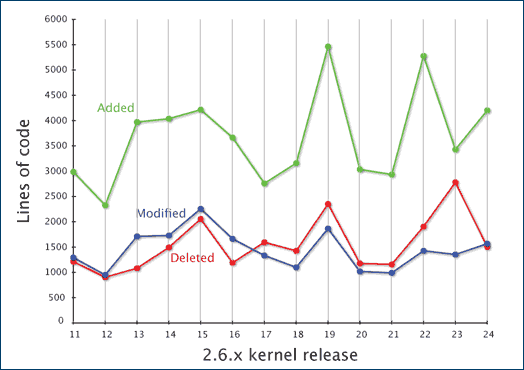
\includegraphics{img/figure5-rateofchange.png}
      }
    \end{figure}
  }

  \subsection{Proporción de código}
  En 2008,
  \begin{itemize}
    \item 9 millones de líneas.
      \begin{itemize}
        \item Drivers: 50-55\%
        \item Kernel: 5\%
      \end{itemize}
    \item Cada año, el código aumenta en un 10\% por igual
      \begin{itemize}
        \item El núcleo del código sigue manteniendo el su proporción del 5\%
      \end{itemize}
  \end{itemize}

  \frame{
    \frametitle{Tamaño por kernel}

    \begin{figure}
      \scalebox{0.35}
      {
        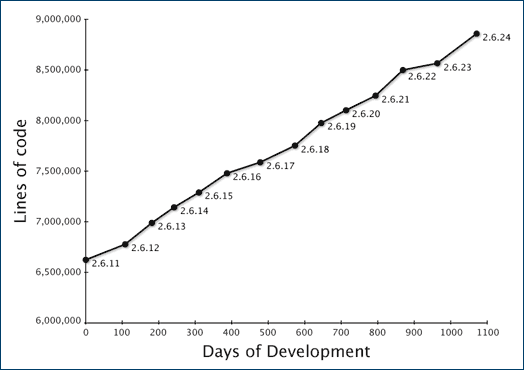
\includegraphics{img/figure4-sizeperkernel.png}
      }
    \end{figure}
  }
  
   \frame{
    \frametitle{Cambios por kernel}

    \begin{figure}
      \scalebox{0.35}
      {
        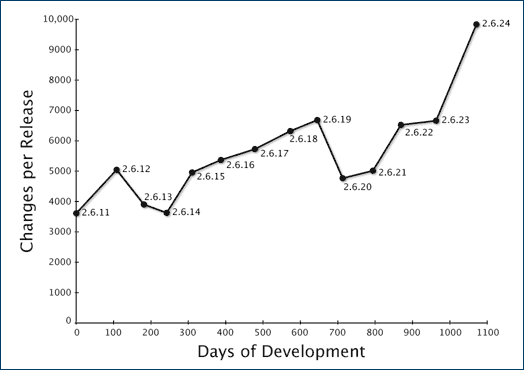
\includegraphics{img/figure2-changesperkernel.png}
      }
    \end{figure}
  }

  \subsection{¿Cómo funciona?}
  \frame{
    \frametitle{$Workflow$}
    \begin{enumerate}
    \item \textbf{Desarrolladores:} 
      \begin{itemize}
      \item Hacen cambios: \textit{bug}, un nuevo driver. 
      \item Se lo manda al \textit{maintainer} (encargado) del archivo, cada archivo tiene uno.
        \begin{itemize}
        \item Cada archivo tiene un encargado
        \end{itemize}
      \end{itemize}
      
    \item \textbf{Mantenedor de archivos:} 
      \begin{itemize}
      \item Revisa los cambios y les da el \textit{visto bueno}
      \item Estos le mandan el archivo a los mantenedores del sub-sistema correspondiente. 
      \item En 2008, existían aproximadamente 600 mantenedores de archivos.
      \end{itemize}
    \end{enumerate}
  }

  \frame{
    \frametitle{$Workflow$}
    \begin{itemize}
    \item \textbf{Mantenedor de sub-sistema:} 
      \begin{itemize}
      \item Última persona en revisar el archivo
      \item Existe un encargado por subsistema
        \begin{itemize}
        \item Seguridad
        \item Redes
        \item Arquitectura ARM
        \item $\vdots$
        \end{itemize}
      \end{itemize}
      
    \item \textbf{Linux $next$ tree:} 
      \begin{itemize}
        \item Todas las noches, Stephen Rothwell hace $pulls$ de los repositorios de cada subsistema
        \item Les hace $merge$
        \item Verifica que compile y pase las pruebas
      \end{itemize}
    \end{itemize}
  }

  \frame{
    \frametitle{$Workflow$}
    \begin{itemize}
    \item \textbf{Releases:} 
      \begin{itemize}
      \item Cada dos semanas se hace un \textit{release candidate (RC)}
        \begin{itemize}
        \item 2.6.19.1.RC1
        \item 2.6.19.1.RC3
        \item $\vdots$
        \end{itemize}
      \item Hasta que Linus Torvalds considere adecuado liberar la versión 2.6.19.1
        \begin{itemize}
          \item Aproximádamente cada $2 \frac{3}{4}$ meses
        \end{itemize}
      \end{itemize}      
    \end{itemize}
  }

  \subsection{¿Quién soporta el trabajo?}
  \frame{
    \frametitle{¿Quién soporta el trabajo?}
    En el a\~{n}o 2008, las entidades que m\'{a}s aportaban al desarrollo del kernel:
    \begin{center}
      \begin{tabular}{|l l l|}
        \hline
        1. & Amateurs (Aficionados) & 18.5\%\\
        2. & Red hat 				  & 11.5\%\\
        3. & IBM 					  & 7.5\%\\
        4. & Novell (Suse)            & 6.6\%\\
        5. & Individuales desconocidos & 5.5\%\\
        6. & Intel 				  & 4.1\%\\
        7. & Oracle 				  & 2.2\%\\
        8. & Consultants 			  & 2.2\%\\
        9. & Academa 				  & 1.5\%\\
        10. & Reneass Technology    & 1.5\%\\
        \hline
      \end{tabular}
    \end{center}
  }
  \section{Market share y usos comunes}

  \frame
  {
    \frametitle{Computadoras personales y netbooks}

    Computadoras personales y portatiles (Junio del 2010)
    \begin{itemize}
      \item Entre el 1\% y 4\% (NetMarket Share y W3C)
      \item Estimado con navegación en la $web$.
    \end{itemize}

    Netbooks
    \begin{itemize}
      \item En 2007, el 90\%. 
      \item En 2009, un tercio (~34\%) de 35 millones de $netbooks$ vendidas.
    \end{itemize}
  }

  \frame{
    \frametitle{Servidores, Mainframes y Supercomputadoras}

    Servidores.
    \begin{itemize}
      \item En el primer cuarto del 2010, el 20\% del mercado (\textit{International Data Corporation}.
      \item Otras otras fuentes con otros métodos de análisis, alegan que ese porcentaje era del 40\%, en el 2009. (Netcraft)
    \end{itemize}

    Mainframes.  
    \begin{itemize}
      \item En 2010, totalmente dominado por el Sistema z de IBM
      \item Red Hat alegaba el 18.4\% en 2007 y el 37\% en 2008.
    \end{itemize}
    
    Supercomputadoras
    \begin{itemize}
      \item Dominado por Linux, en un 91\%.
      \item Unix (4.40\%).
    \end{itemize}
  }

\end{document}
